\clearpage

\section{Evaluation}
\nblink{brats/05\_evaluate.ipynb}

After training the neural network, we investigated the quality of the neural network with a graphical representation. Figure \ref{brats_evaluation}
shows the ground truth generated by the preprocessing step on the left side and the output generated by our network on the right side.

\begin{figure}[H]
    \centering
    \begin{subfigure}[t]{.5\textwidth}
        \centering
        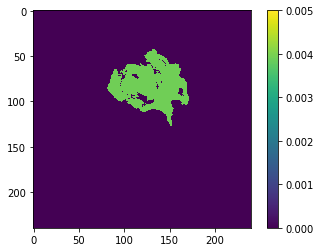
\includegraphics[width=\linewidth]{chapters/04_segmentation/images/evaluate1.png}
        \caption{Ground truth segment from dataset}
    \end{subfigure}%
    \begin{subfigure}[t]{.5\textwidth}
        \centering
        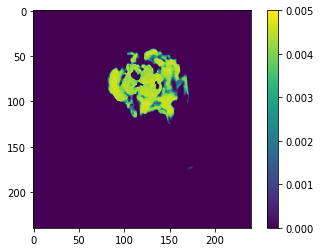
\includegraphics[width=\linewidth]{chapters/04_segmentation/images/evaluate2.png}
        \caption{Output from trained neural network (floating point values, not binarized)}
    \end{subfigure}
    \caption{Comparing the neural network output with the dataset ground truth shows a high correlation.}
    \label{brats_evaluation}
\end{figure}

As a second visualization, we generated a confusion matrix between the ground truth and the binarized network output (Figure \ref{brats_confusion_matrix}).
We binarized the network output by blacking out all pixels below the mean of the image, and making all pixels white which are above the mean.

\begin{figure}[H]
\centering
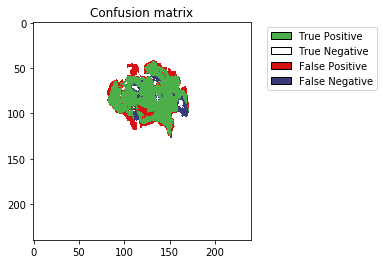
\includegraphics[width=10cm]{chapters/04_segmentation/images/confusion_matrix.png}
\caption{Confusion matrix visualization comparing the binarized network output with the ground truth segment. This confirms the high correlation between output and ground truth}
\label{brats_confusion_matrix}
\end{figure}
